\documentclass[UTF8]{ctexart}

\usepackage{subfiles}  

%下面的语句, 引入你的头部设置文件
\usepackage{C:/phpStorm_proj/02_myself_ID_EGO/+100_latex_all_math_sel/myPreamble} 
%必须是绝对路径,才能让各个tex在单独编译时使用到

\title{文件名}


%---------------------------------


\begin{document}
	\tableofcontents % 生成目录
	\date{} % 若不写这句, 则默认也会渲染出日期, 所以我们要手动赋空值
	\maketitle  %这行代码, 让你前面的 title, author, date生效
	
	\part{幂律分布 Power law distribution}
	
	\section{幂律分布: 在随机变量中,越小的数值,出现的概率越大; 越大的数值,出现的概率则越小}
	
	幂律分布的``概率(密度)函数 f(x)"是: $\boxed{
		f(x)= cx^{-\alpha -1}, \quad  x \to \infty
	}$ ← $\alpha$是参数. \\

	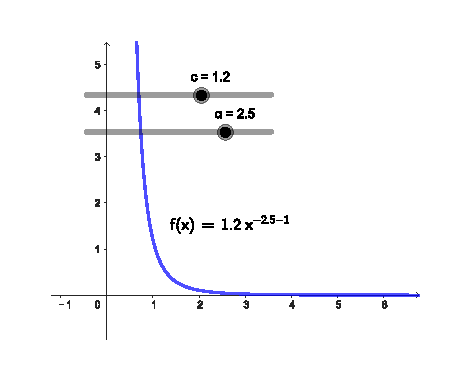
\includegraphics[width=0.5\textwidth]{/0229.pdf} \\

	幂律分布的``互补累积分布函数 F(x)"(CCDF) 是: $\boxed{	P(X \geq x)=cx^{-\alpha}, \quad  x \to \infty }$ \\
	
	注意: CDF 和 CCDF 的区别:  \\
	\begin{tabular}{|p{0.5\textwidth}|p{0.5\textwidth}|}
		\hline
		累积函数 CDF (Cumulative Distribution Function) &   $F_X(x)=P(X\leq x)$\\
		\hline
		互补累计函数 CCDF (Complementary Cumulative Distribution Function) & $F(a)=P(x>a)$. 注意, 这里是大于号(>)! \\
		\hline
	\end{tabular} \\

	
	在统计学中,幂律 power law 表示的是两个量之间的函数关系: 其中一个量的相对变化, 会导致另一个量的相应``幂次比例"的变化,且与初值无关. \\
	
	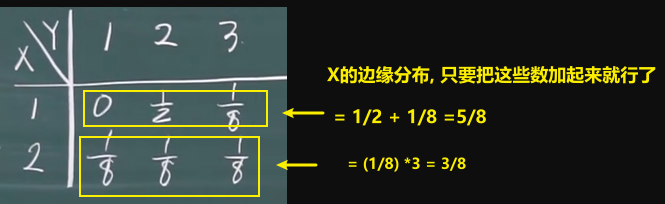
\includegraphics[width=0.6\textwidth]{/0228.png} \\
	
	曲线的横坐标,代表随机变量的取值; 纵坐标,代表发生的概率. \\
	\textbf{幂律分布曲线的含义非常明确 : 在随机变量中,越小的数值, 出现的概率越大; 越大的数值,出现的概率则越小.} \\
	
	
	
	\begin{myEnvSample}
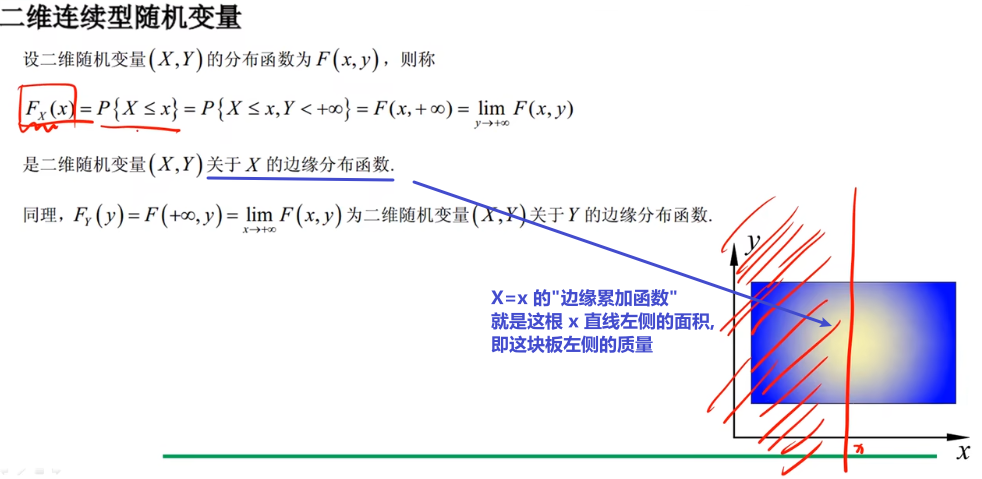
\includegraphics[width=1\textwidth]{/0239.png} \\

→ 上面的图b (高速公路网), 是泊松分布. 每个城市有数量相对均衡的高速公路,不会出现连接上百条高速公路到同一个城市的; 也没有哪个城市一条高速公路都没有. 多数城市非常相似。 \\
其直方图, 就呈现为一条钟形曲线(a图). 这种相对均匀分布的属性, 即为``正态分布; 泊松分布". 是随机网络固有的性质. \\

\textbf{泊松分布有一个明显的峰值},表明大多数节点所拥有的链接数, 和节点拥有的``平均链接数"一样. 在峰值的两侧,钟形曲线呈``指数级骤减",处于平均线之外的异常个体, 几乎不存在. \\

→ 图d, 是航空交通网络. 大多数飞机场都很小,只有几个航班。同时,也有少量非常大的机场,这样的枢纽节点连接着上百个小机场。这种分布对应着``幂律分布"(图c). \\

		
	\textbf{``幂律分布"没有峰.} 其直方图是不断递减的曲线,\textbf{在线的两端可以无限逼近和延伸. 幂律最突出的特征是: 大量微小事件, 和少数非常重大的事件, 并存.} \\
	
	
	
	\underline{网络中, 新加入的节点, 是如何与原有的节点, 产生链接的? } \\	
	\textbf{如果新节点是``随机地"选择与其他节点进行连接,那么真实世界将符合``正态分布").} \\
	\textbf{然而, 在大多数真实网络中,新加入的节点, 更倾向于与链接数高的节点相连,这个过程被称为``偏好连接”。这就会导致``超级枢纽节点"出现.} \\
	我们倾向于建立的连接, 都不是普通的节点,而是``枢纽节点"。他们越出名,指向他们的链接就越多(广告效应, 富者愈富, 马太效应)。这些节点, 就形成了网络中链接数较多的节点, 成为枢纽。 \\
	
	- 如果是70亿人随机匹配约会对象,贝克汉姆可能永远也无法匹配到另一个影视巨星。 \\
	- ``六度分隔理论”, 背后并不是指每个人都认识差不多数量的人,大家彼此均衡地组成人际网络,所以互相认识。\textbf{而是极少数的超级社交达人(起着中枢作用),将多个分割的人际网络岛屿, 联系了起来.} \\
	- 投资公司Horsley Bridge在1985年到2014年间, 投资了7000家初创企业,其中仅占5\%的一小部分投资,创造了其全部回报的60\%。 \\
	- 少数公司大获成功一发不可收拾,大部分公司则历经挫折一败涂地。 
		\end{myEnvSample}
	
	
	
	
	\section{性质}
	
	\subsection{尖峰肥尾} 
	
	- 尖峰 : 说明有些x的值很小(赚1000元/月), 但其数量规模大到超乎想象(6亿人). \\
	- 肥尾 : 说明很多极小概率事件(世界首富), 依然有可能发生. \\
	
	\textbf{幂律分布, 会让原本不会发生的极端事件发生.} 在数学上,这个叫``长尾”,也叫肥尾、厚尾. 就是说: \textbf{虽然极端数据出现的概率很低,但这个概率永远不会趋近于0},永远不会小到可以忽略不计.  \\
	
	在``正态分布"里, 数据非常集中于平均值附近,非常极端的数据几乎不可能出现. 而在``幂律分布"里, 再极端的数据都有出现的可能. \\	
	超大规模的自然灾害, 虽然发生概率极低, 但我们知道它一定会发生. \textbf{在幂律分布里,极端数据往往意味着极端事件.} \\
	
	
	如果人的身高, 是符合``幂率分布"的话, 则就会有极少数``身高能长到数公里"的人存在. 
	
	
	
	\subsection{无标度 -- 分形效果}
	
	无标度,也叫``无尺度”, ``尺度无关”. 意思是: 在任何观测尺度下,``幂律分布"都呈现同样的分布特征. 即, 无论你从曲线上截取哪一段, 是长是短, 它都含有二八定律存在(虽然曲率不同). 就相当于``分形"效果. \\	
	一般的分布, 都会有个尺度范围,在这个范围内服从这个分布,超过这个尺度可能就不服从这种分布了。而``幂律分布"没有尺度的限制,不管截取任何一个部分,都仍然呈现幂律分布的特征. \\
	
	比如,图书销量是服从``幂律分布"的 : \\
	- 最畅销那本书的销量, 在前10名销量中占的比例, \\
	- 和前10名的销量, 在前100名的销量中占的比例, \\
	- 和前100名, 在前1000名的总销量中占的比例,\\
	大体都是相同的. 这就是``幂律分布"唯一的数学特征——无标度.
	
	
	
	\subsection{幂律分布让``均值$\mu$"失去意义} 
	
	``正态分布"是一种均匀对称分布, 大多数数据都集中在``均值 $\mu$"附近, 所以均值非常有用, 因为它代表大多数. \\	
	而\textbf{``幂律分布"呢? 它的数据变化幅度非常大,平均值毫无意义.} 比如个人收入,有穷人,也有富豪,把这两群人的资产平均 (人均收入),毫无意义. 
	
	
	
	\subsection{幂律分布中的``波动性(方差$\sigma$)"失去意义}
	幂律分布,随机变量波动的范围非常大,常用的``平均值"、``标准差"到这里都没用了. 
	
	
	
	\subsection{符合``幂律分布"的事件, 其何时发生, 和发生的规模, 完全不可预测}
	符合``幂律分布"的事件, 必定发生大事件, 但无法对其的发生进行预测. \\
	
	- 如``沙堆模型”: 随着沙堆高度的增加,新添加的沙粒会带动沙堆表面其他沙粒滚落,产生``沙崩”。经过统计沙崩的规模和发生的频率,人们发现该事件服从``幂律分布"。但是, 我们既不知道在什么条件下,再放一粒沙子就会导致沙崩; 也无法预测这粒沙子导致的沙崩规模, 会有多大。 \\
	- 	同理, 我们对于幂律分布的事物,比如各种自然灾害,预报上基本还是束手无策。
	我们知道大灾一定会来, 但我们不知道下一场大地震、下一场战争、下一次金融危机会什么时候发生,以及会带来多大的损失.  \\
	
	
	你可能会说,不是有``二八法则"吗? 我们抓重点,抓住重要的20\%不就好了吗? 但这是个``存量思维",可以总结``过去",但无法预测``未来". \textbf{虽然我们知道80\%的生意来自于20\%的客户,但你永远不知道下一个客户是属于重要的20\%,还是不重要的80\%。} \\
	
	
	
	
	\subsection{在``双对数坐标系"下,幂律分布表现为一条斜率为``幂指数的负数"的直线}
	
	自然界中大多数被识别的幂律的指数是这样的:平均值是明确的,但方差不是. 这意味着它们能够出现黑天鹅行为. \\
	
	关于坐标系: \\
	(1) 算术坐标系统(笛卡儿坐标) : 横,纵的刻度, 都是是等距的. \\
	
	(2) ``对数"坐标系统 : \textbf{坐标轴是按照``相等的指数增长变化"表示的.} 举例来说:如果每1cm 代表10的1次方增加,则坐标轴刻度的表示依次为: 1,10,100,1000,10000 ... \\
	
	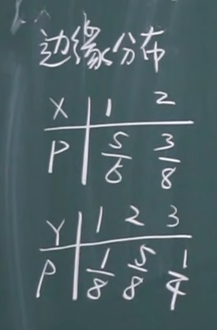
\includegraphics[width=1\textwidth]{/0230.png} \\
	
	
	
	
	
	(3) ``双对数"坐标: 指两个坐标轴, 都是``对数坐标". 即假如对应于x、y轴,则两轴等刻度情况下,其值``以相应底数, 成次方增长". (注意:在各自坐标轴上的是``真数",不是求对数后的值.) 
	
	
	
	
\subsubsection{什么时候, 要使用到``对数"坐标系呢?}  
	→ 如果所研究的函数的y值, 和自变量x, 在数值上均变化了几个数量级. 比如,已知x和y的数据为:x= 10, 20, 40, 60, 80, 100, 1000, 2000, 3000, 4000  y= 2, 14, 40, 60, 80, 100, 177, 181, 188, 200. 则, 在``直角坐标系"上, 就很难作图. 而换用``对数坐标系", 就能够画出来. \\
	→ \textbf{当需要变换某种``非线性关系"为``线性关系"时.} (比如, ``幂率分布"的概率函数(幂函数)图上.) \\
	
	
	\begin{myEnvSample}
	比如, $1 \leq x \leq 10000, \ y=lg(x^2)$ 这个函数,直接画图, 会是这样: \\
	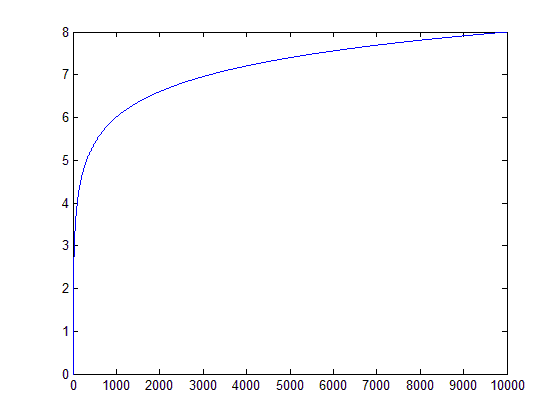
\includegraphics[width=0.55\textwidth]{/0232.png} \\
	
	→ x是10000时, y输出 : $
	\lg \left( 10000^2 \right) =\underset{\text{即问:}10^?=10^8,\text{显然指数是}8}{\underbrace{\log _{10}\left( 10^4 \right) ^2}}=8
	$ \\
	→ x是1000时, y输出 : $
	\lg \left( 1000^2 \right) =\underset{\text{即问:}10^?=10^3,\text{显然指数是}6}{\underbrace{\log _{10}\left( 10^3 \right) ^2}}=6
	$ \\
	
	我们采用``对数坐标系": 让 x 采用``对数标度", y 轴仍保持``线性标度". 从这种图中就可以看出, 函数 $y=lg(x^2)$ 本质上是一个``线性函数": \\
	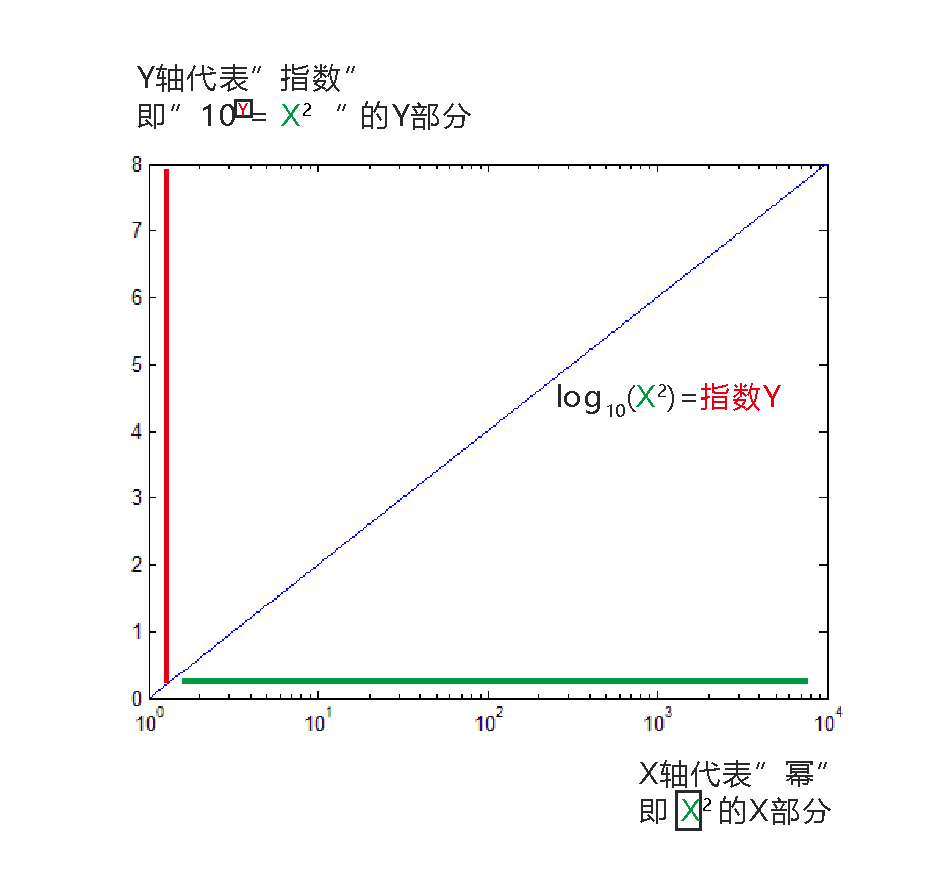
\includegraphics[width=0.7\textwidth]{/0233.pdf} 
	\end{myEnvSample}
\vspace{1em} 
	

	\begin{myEnvSample}
		摩尔定律说: 晶体管和其他电子元件的数量, 每2年会翻一番. \\
		以年份作为x轴,芯片中的晶体管数量作为y
		轴,摩尔定律描述的曲线大概是这样的: \\
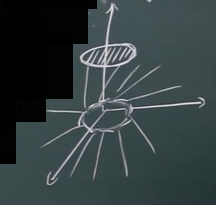
\includegraphics[width=0.55\textwidth]{/0235.png} \\		
		
		
	数据点呈``指数型"增长,需要我们用 $y=ce^{ax}$ 这样的``指数函数"去拟合. 然而实际上,手工计算你将得不到最佳拟合曲线,因为解方程会十分困难. \\
		
如果纵坐标取``对数坐标轴",会得到:\\
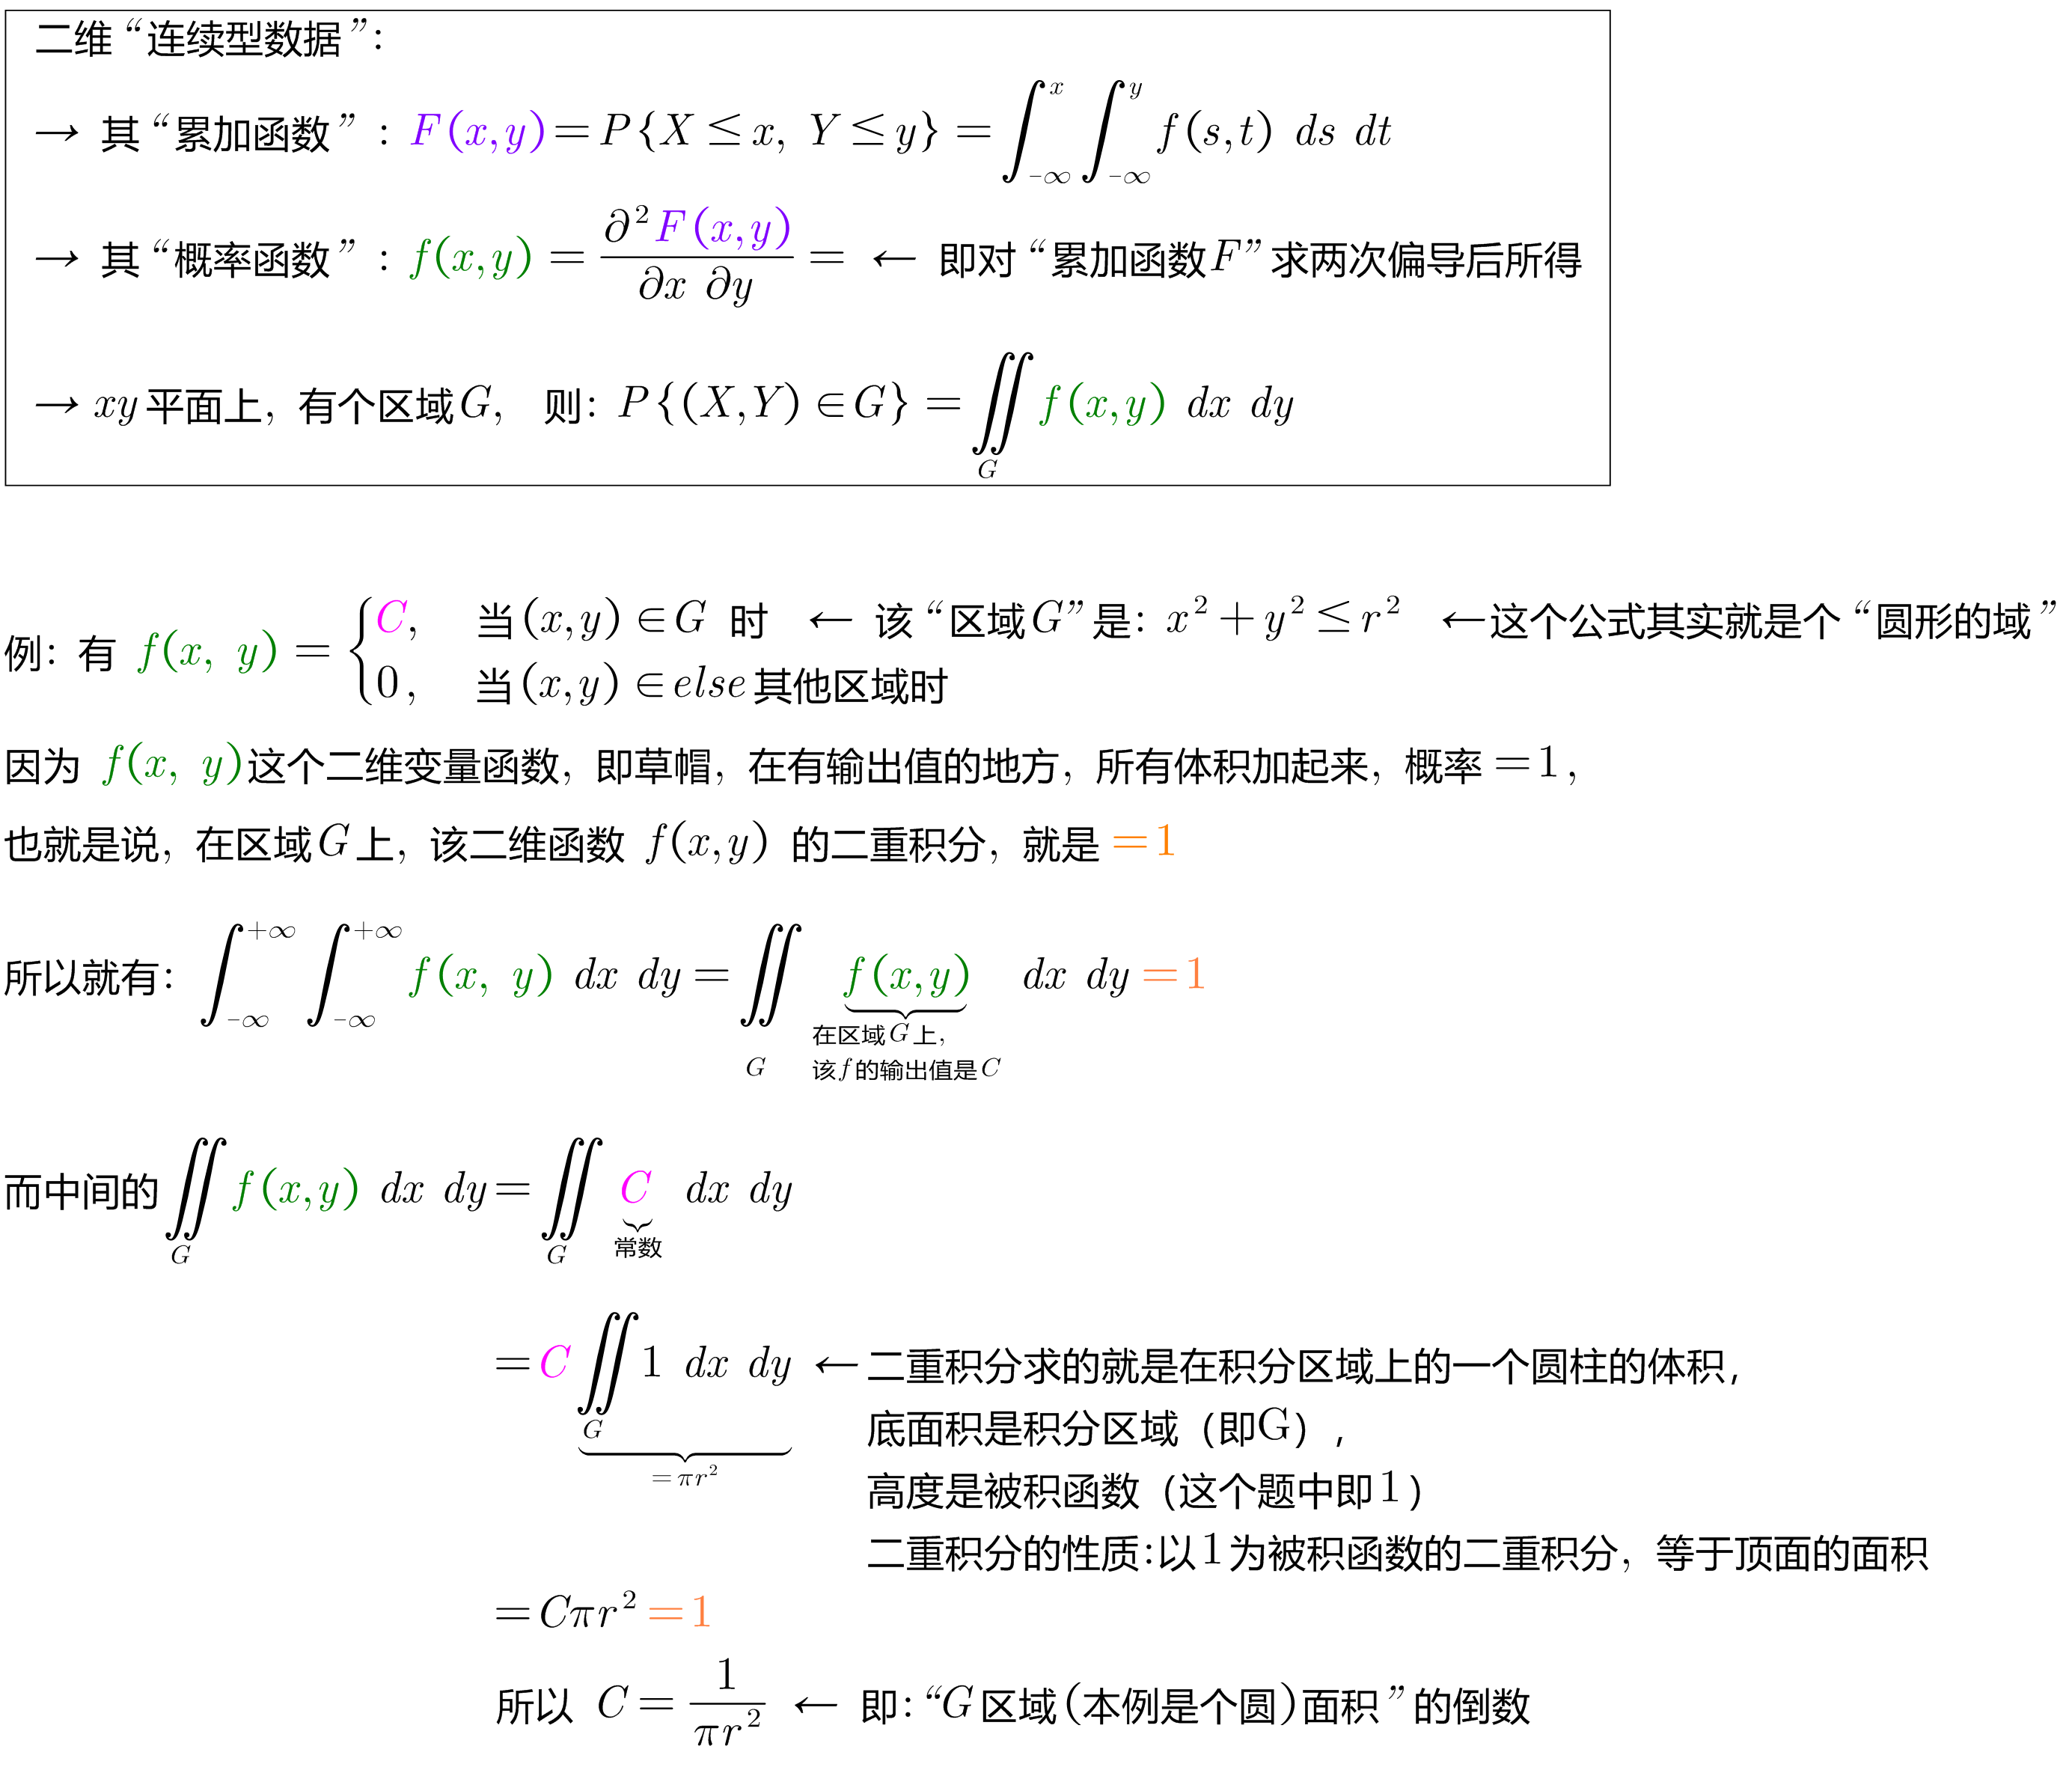
\includegraphics[width=0.5\textwidth]{/0234.png} \\
看上方的一系列点,它们呈现``线性增加"的趋势. \\

将 $y=ce^{ax}$ 两边, 同时取对数, 会得到: \\
$
\lg y=\lg (ce^{ax})=\lg c+\lg e^{ax}=\lg c+ax\lg e=\lg c+(a\lg e)x
$ \\

式子中有 a 和 lg(c) 两个未知数. 用``最小二乘法"可以得到最佳拟合直线,从而可以预测未来芯片中, 晶体管的数量. 
	\end{myEnvSample}
\vspace{1em} 




\begin{myEnvSample}
八大行星到太阳的平均距离, 以及它们各自的公转周期,由此算出角速度和向心加速度: \\
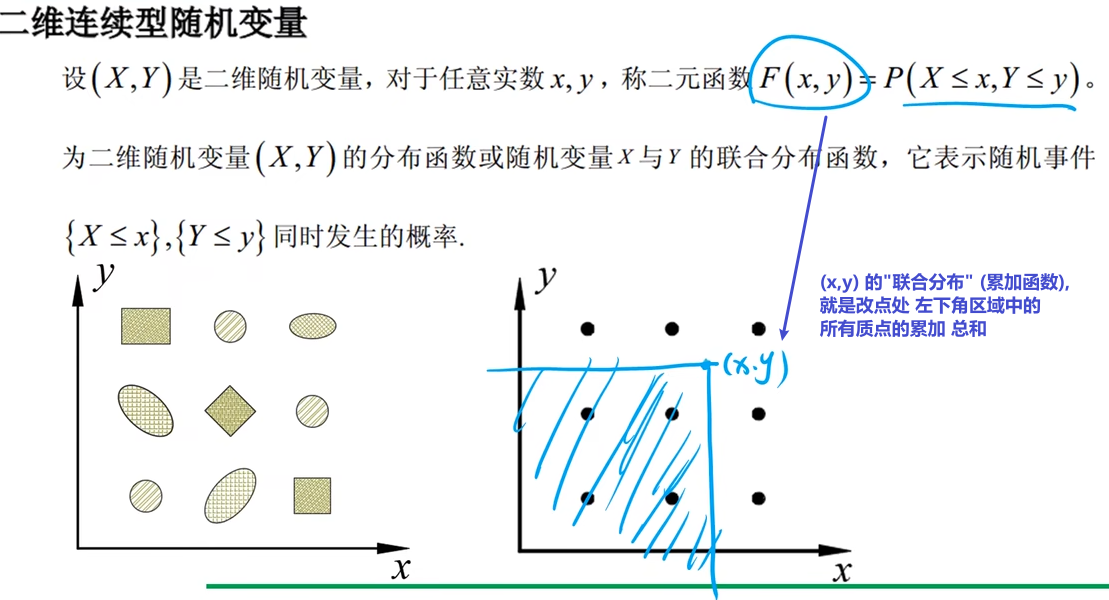
\includegraphics[width=0.6\textwidth]{/0236.png} \\

看第一列和最后一列,以平均距离R 为x轴; 加速度a 为y轴, 来绘制图像: \\

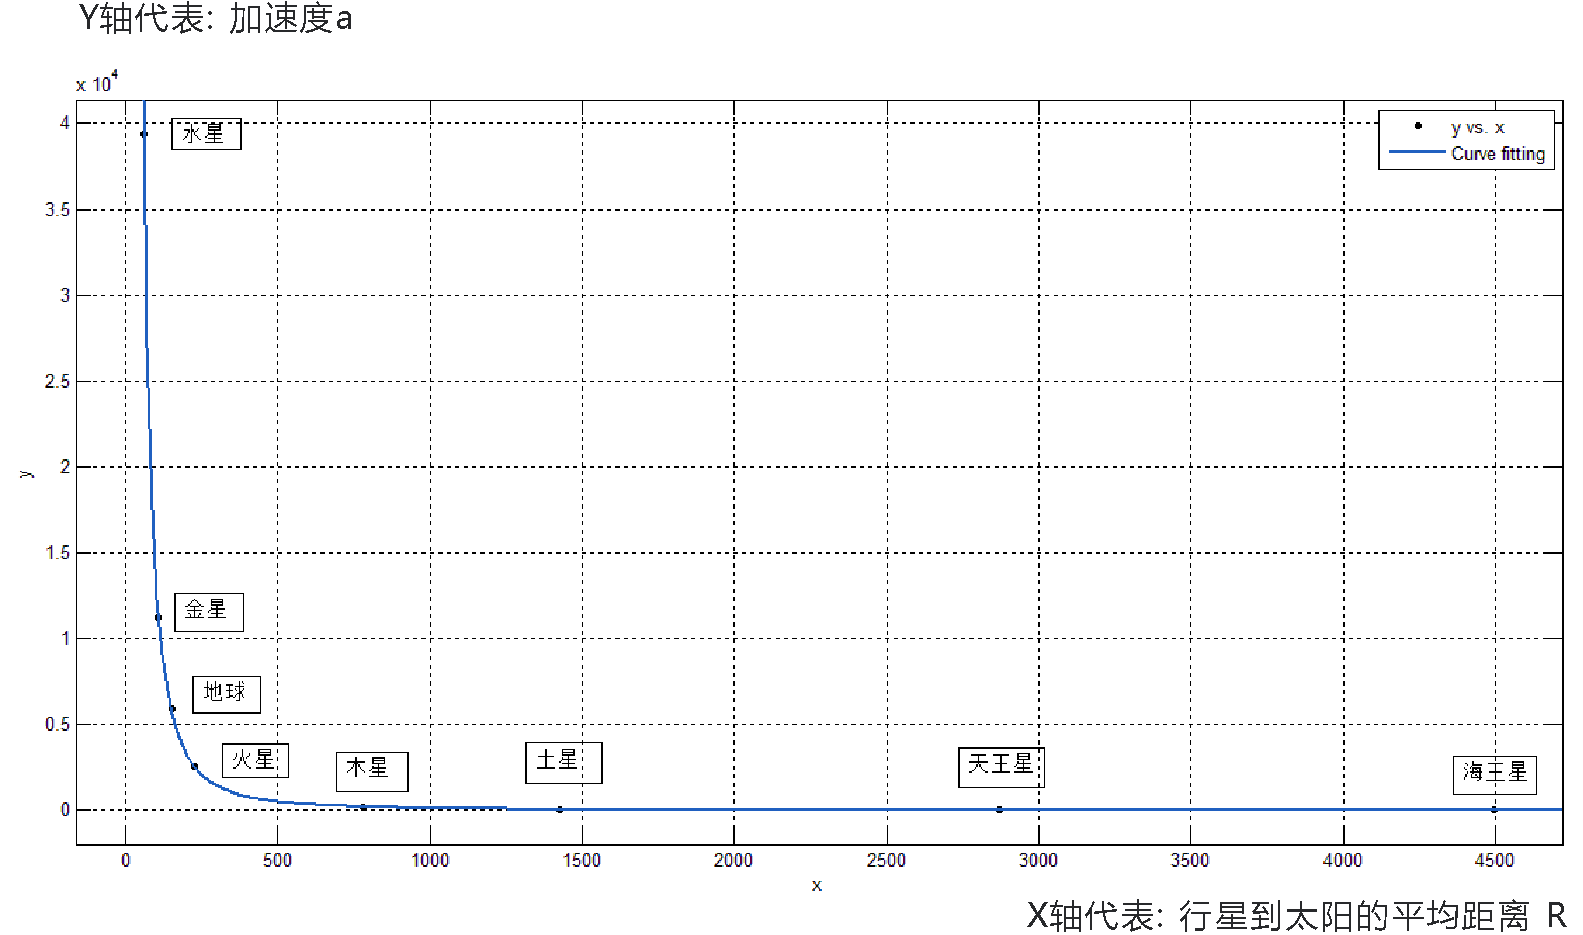
\includegraphics[width=1\textwidth]{/0237.pdf} \\

当然现在,我们还看不出x和y的关系. 但是对两个坐标轴``取对数"后,图像就是: \\
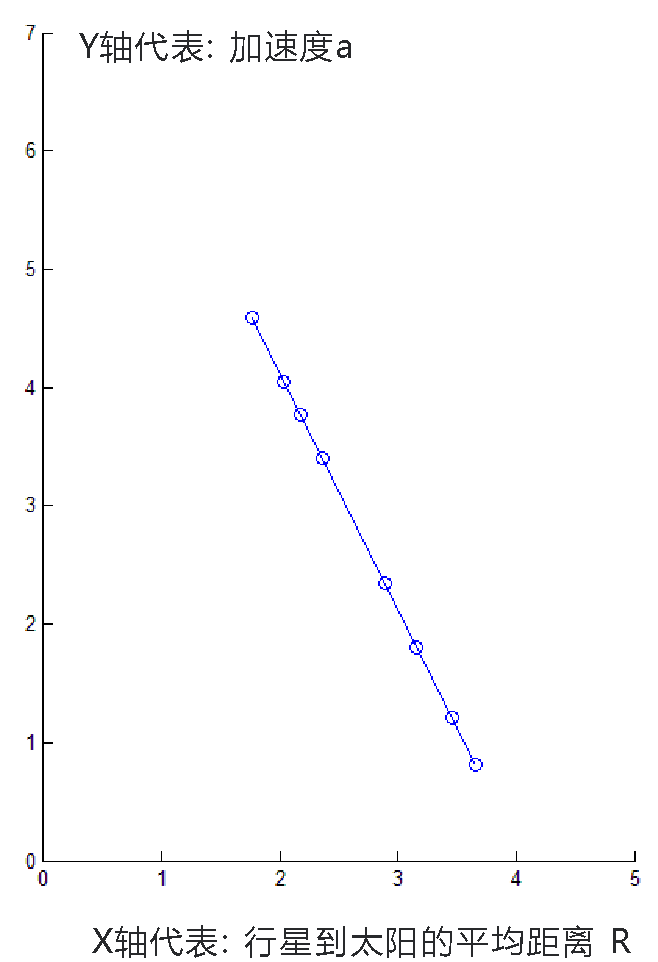
\includegraphics[width=0.35\textwidth]{/0238.pdf} \\

数据点落在了一条直线上!该直线的斜率大约是 −2.  也就是说: 该直线的方程为: \\
$
\underset{y}{\underbrace{\lg a}}=\underset{\text{斜率}k}{\underbrace{-2}}\lg \underset{x}{\underbrace{R}}+\underset{b,\text{即直线在}y\text{轴上的截距}}{\underbrace{\lg p}}
$ \\
因此: 
\begin{align*}  % 支持每行编号. 若不需要编号, 就用 align*环境
	&\lg a=-2\lg R+\lg p\\
&\lg a=\lg (R)^{-2}+\lg p\\
&\lg a=\lg (R^{-2}\cdot p)\\
&\text{即}a=R^{-2}\cdot p=\frac{p}{R^2}
\end{align*}

或者说: $a\underset{\text{正比于}}{\underbrace{\propto }}\frac{1}{R^2}$ \\

$\propto $ 这个符号是``正比于"的意思. 也就是说 : \textbf{两个变量具备相同的递增递减性, 并且近似于``线性关系". ``正比”的字面含义就是两个变量是``1次幂"的的关系,且``比值"为正的常数.} 如果两个变量不是线性关系, 数学上就一般不用``正比"来表达. \\
形如 Y=KX 的函数, 其中K为非零参数, Y与X就叫``成正比".  \\

本例说明, 各行星的``向心加速度a", 和``其到太阳距离(R)"的平方, 成反比!即: $a=p \cdot \dfrac{1}{R^2}$  \\
向心加速度, 是由万有引力引起的,因此推测引力 F 与 $R^2$ 成反比, 也是合理的 (事实也的确如此). 
\end{myEnvSample}





	\subsubsection{真数 : 即 $\boxed{\text{底}^{\text{指}(\text{真数})}=\text{幂}}$中的``指数"}
	什么是``真数 natural(number); antilogarithm"? \\
	即: $
	\underset{\text{底}}{\underbrace{2}}\overset{\text{指,对数}}{\overbrace{^3}}=\overset{\text{幂,真数}}{\overbrace{8}},\ \text{即\ }\log _{\underset{\text{底}}{\underbrace{2}}}\overset{\text{幂,真数}}{\overbrace{8}}=\overset{\text{指,对数}}{\overbrace{3}}
	$ ) \\
	
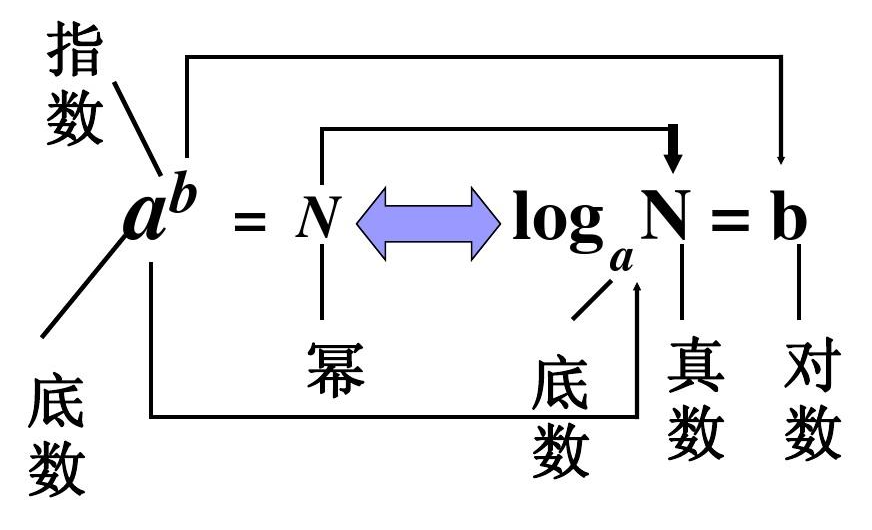
\includegraphics[width=0.35\textwidth]{/0231.png} \\




	\subsection{幂律分布可是我们对抗``熵增"的中间经过状态}	
	水在变成冰的过程中,存在一个临界温度 --- 在临界温度之前, 水分子里原子的自旋, 都是随机指向不同的方向的; 可一旦到了临界温度,就会非常有序地指向同一个方向. \\	
	1982年诺贝尔物理学奖得主 肯尼斯·威尔逊, 收集了很多临界态 ---  ``瞬间"的关键数据. 结果发现: 每个指标都在临界态附近, 涌现出了幂律分布。 我们知道,\textbf{无序是嫡值最大,有序是嫡值最小. 这说明,从无序到有序这个``减嫡"的过程, 和``幂律分布"有着相关关系。 这可能意味着, 幂律分布是我们对抗``熵增"的经过状态.} 
	
	
		
	
	
	
\end{document}